% ------------------------------------------------------------------------
% ------------------------------------------------------------------------
% Monografia Peacon
% Trabalho de Conclusão de Curso
% Baseia-se no documento modelo de TCC do abntex2
% Para saber mais, acesse https://github.com/abntex/abntex2
% ------------------------------------------------------------------------
% ------------------------------------------------------------------------

\documentclass[
		% -- opções da classe memoir --
		12pt,				% tamanho da fonte
		openright,			% capítulos começam em pág ímpar (insere página vazia caso preciso)
		oneside,			% para impressão em verso e anverso. Oposto a oneside
		a4paper,			% tamanho do papel. 
		% -- opções da classe abntex2 --
		chapter=TITLE,		% títulos de capítulos convertidos em letras maiúsculas
		%section=TITLE,		% títulos de seções convertidos em letras maiúsculas
		%subsection=TITLE,	% títulos de subseções convertidos em letras maiúsculas
		%subsubsection=TITLE,% títulos de subsubseções convertidos em letras maiúsculas
		% -- opções do pacote babel --
		english,			% idioma adicional para hifenização
		brazil				% o último idioma é o principal do documento
	]{abntex2}


% ----------------------------------------------------------
% Pacotes básicos 
% ----------------------------------------------------------
%\usepackage{helvet}			
\usepackage[scaled]{helvet}
\renewcommand*\familydefault{\sfdefault} 	% Only if the base font of the document is to be sans serif
										% Foi necessário para acertar o documento, continha diversos erros
\usepackage[T1]{fontenc}		% Selecao de codigos de fonte.
\usepackage[utf8]{inputenc}	% Codificacao do documento (conversão automática dos acentos)
\usepackage{lastpage}		% Usado pela Ficha catalográfica
\usepackage{indentfirst}		% Indenta o primeiro parágrafo de cada seção.
\usepackage{color}			% Controle das cores
\usepackage{graphicx}		% Inclusão de gráficos
\usepackage{microtype} 		% para melhorias de justificação
% ----------------------------------------------------------
		

% ----------------------------------------------------------
% Pacotes adicionais, usados apenas no âmbito do Modelo Canônico do abnteX2
%% ----------------------------------------------------------
\usepackage{lipsum}				% para geração de dummy text
\usepackage{customizacoes} 		% customizações feitas pelo autor
% ----------------------------------------------------------


% ----------------------------------------------------------
% Pacotes de citações
% ----------------------------------------------------------
\usepackage[alf]{abntex2cite}				% Citações padrão ABNT

% ----------------------------------------------------------
% CONFIGURAÇÕES DE PACOTES
% ----------------------------------------------------------

% ----------------------------------------------------------
% Configurações do pacote backref
% ----------------------------------------------------------
\definecolor{thered}{rgb}{0.65,0.04,0.07}
\definecolor{thegreen}{rgb}{0.06,0.44,0.08}
\definecolor{thegrey}{gray}{0.5}
\definecolor{theshade}{rgb}{1,1,0.97}
\definecolor{theframe}{gray}{0.6}
% ----------------------------------------------------------



% ----------------------------------------------------------
% Informações de dados para CAPA e FOLHA DE ROSTO
% ----------------------------------------------------------

\titulo{Iris - Segundo Trabalho}
\autor{Karoline Kimiko Figueiredo Setoue}
\local{Bauru}
\data{2017}
%\orientador{Prof. Dr. Kelton Augusto Pontara da Costa}
%\coorientador{Prof. Dr. João Paulo Papa}
\instituicao{%
  Universidade Estadual Paulista "Júlio de Mesquita Filho"
  \par
  Pós-Graduação em Ciência da Computação
}
\tipotrabalho{Monografia (Trabalho de Conclusão de Curso)}
% O preambulo deve conter o tipo do trabalho, o objetivo, 
% o nome da instituição e a área de concentração 
% foi necessário utilizar \~{a} e etc para os acentos por problemas na geração do PDF
%\preambulo{Trabalho de Conclus\~{a}o do Curso de Bacharelado em Ciência da Computação apresentado ao Departamento de Computa\c{c}\~{a}o da Faculdade de Ci\^{e}ncias da Universidade Estadual Paulista ``J\'{ú}lio de Mesquita Filho'' – UNESP, C\^{a}mpus de Bauru.}

% ----------------------------------------------------------


% ----------------------------------------------------------
% Configurações de aparência do PDF final
% ----------------------------------------------------------

% alterando o aspecto da cor azul
\definecolor{blue}{RGB}{0,0,0}

% informações do PDF
\makeatletter
\hypersetup{
     	%pagebackref=true,
		pdftitle={\@title}, 
		pdfauthor={\@author},
    	pdfsubject={\imprimirpreambulo},
	    pdfcreator={LaTeX with abnTeX2},
		pdfkeywords={Redes Neurais Artificiais}{Computação em Nuvem}{Balanceamento de cargas}{abntex2}{trabalho acadêmico}, 
		colorlinks=true,       		% false: boxed links; true: colored links
    	linkcolor=blue,          	% color of internal links
    	citecolor=blue,        		% color of links to bibliography
    	filecolor=magenta,      		% color of file links
		urlcolor=blue,
		bookmarksdepth=4
}
\makeatother
% ----------------------------------------------------------


% ----------------------------------------------------------
% Espaçamentos entre linhas e parágrafos 
% ----------------------------------------------------------

% O tamanho do parágrafo é dado por:
\setlength{\parindent}{1.3cm}

% Controle do espaçamento entre um parágrafo e outro:
\setlength{\parskip}{0.2cm}  % tente também \onelineskip

% ----------------------------------------------------------
% compila o indice
% ----------------------------------------------------------
\makeindex
% ----------------------------------------------------------


% ----------------------------------------------------------
% Configurações de projeto
% ----------------------------------------------------------
\newif\iffinal
\finaltrue % define se é um arquivo final, se for não for retira umas partes. 

\newif\ifrelatorio
\relatoriofalse % define se é um arquivo final, se for não for retira umas partes. 

\newif\ifabstract
\abstractfalse % define se mostra o abstract em inglês ou não.

\newif\ifresumo
\resumotrue % define se mostra o resumo ou não.

\newif\ifficha
\fichafalse % define se mostra a ficha catalográfica ou não
% ----------------------------------------------------------


% ----------------------------------------------------------
% Início do documento
% ----------------------------------------------------------
\begin{document}

% Seleciona o idioma do documento (conforme pacotes do babel)
%\selectlanguage{english}
\selectlanguage{brazil}

% Retira espaço extra obsoleto entre as frases.
\frenchspacing 

% ----------------------------------------------------------
% ELEMENTOS PRÉ-TEXTUAIS
% ----------------------------------------------------------
\pretextual


% ----------------------------------------------------------
% Capa
% ----------------------------------------------------------
\imprimircapa
% ----------------------------------------------------------


% ----------------------------------------------------------
% Folha de rosto
% (o * indica que haverá a ficha bibliográfica)
% ----------------------------------------------------------
%\imprimirfolhaderosto
% ----------------------------------------------------------


% ----------------------------------------------------------
% Inserir a ficha catalográfica
% ----------------------------------------------------------

% Isto é um exemplo de Ficha Catalográfica, ou "Dados internacionais de
% catalogação-na-publicação''. Você pode utilizar este modelo como referência. 
% Porém, provavelmente a biblioteca da sua universidade lhe fornecerá um PDF
% com a ficha catalográfica definitiva após a defesa do trabalho. Quando estiver
% com o documento, salve-o como PDF no diretório do seu projeto e substitua todo
% o conteúdo de implementação deste arquivo pelo comando abaixo:
%
% \begin{fichacatalografica}
%     \includepdf{fig_ficha_catalografica.pdf}
% \end{fichacatalografica}

%\begin{fichacatalografica}
%	\sffamily
%	\vspace*{\fill}					% Posição vertical
%	\begin{center}					% Minipage Centralizado
%		\fbox{\begin{minipage}[c][8cm]{13.5cm}		% Largura
%				\small
%				\imprimirautor
%				%Sobrenome, Nome do autor
%				
%				\hspace{0.5cm} \imprimirtitulo / \imprimirautor. --
%				\imprimirlocal, \imprimirdata-
%				
%				\hspace{0.5cm} \pageref{LastPage} p. : il. (algumas color.) ; 30 cm.\\
%				
%				\hspace{0.5cm} \imprimirorientadorRotulo~\imprimirorientador\\
%				
%				\hspace{0.5cm}
%				\parbox[t]{\textwidth}{\imprimirtipotrabalho~--~\\ \imprimirinstituicao,
%					\imprimirdata.}\\
%				
%				\hspace{0.5cm}
%				1. Balanceamento de Cargas.
%				2. Redes Neurais Artificiais.
%				3. Computação em Nuvem.
%				I. \imprimirorientador.
%				II. Universidade Estadual Paulista "Júlio de Mesquita Filho".
%				III. Faculdade de Ciências.
%				IV. \imprimirtitulo
%			\end{minipage}}
%		\end{center}
%	\end{fichacatalografica}
%
%\begin{fichacatalografica}
%	\ttfamily
%	\vspace*{\fill}					% Posição vertical
%	\hspace{1.5cm}
%	\begin{centering}	% Minipage Centralizado
%		\fbox{\begin{minipage}[c][7.5cm]{12.5cm}		% Largura
%				\footnotesize
%				\vspace{0.3cm}
%				\hspace{2.0cm} Setoue, Karoline Kimiko Figueiredo.
%				%Sobrenome, Nome do autor
%				
%				\hspace{2.0cm} \parbox[t]{\textwidth}{\hspace{0.5cm} Aplicação de redes neurais artificiais no balanceamento de carga em serviços de nuvem / \imprimirautor, \imprimirdata} 	\\	
%				
%				\hspace{2.0cm} \parbox[t]{\textwidth}{\hspace{0.5cm} \pageref{LastPage} f. : il.} \\
%				
%				\hspace{2.0cm} \parbox[t]{\textwidth}{\hspace{0.5cm} \imprimirorientador} \\
%				
%				\hspace{2.0cm} \parbox[t]{\textwidth}{\hspace{0.5cm} Monografia (Graduação)~--~Universidade Estadual \\ Paulista. Faculdade de Ciências, Bauru, 2017 \\}  
%				\\	
%				
%				
%				\hspace{2.0cm} \parbox[t]{\textwidth}{\hspace{0.5cm} 1. Balanceamento de carga. 2. Redes neurais artificiais. \\ 3. Computação em nuvem. I. Universidade \\ Estadual Paulista. Faculdade de Ciências. II. Título.}	
%			\end{minipage}}
%		\end{centering}
%	\end{fichacatalografica}
% ----------------------------------------------------------


% ----------------------------------------------------------
% Inserir errata
% ----------------------------------------------------------
%\begin{errata}
%Elemento opcional da \citeonline[4.2.1.2]{NBR14724:2011}. Exemplo:

%\vspace{\onelineskip}

%FERRIGNO, C. R. A. \textbf{Tratamento de neoplasias ósseas apendiculares com
%reimplantação de enxerto ósseo autólogo autoclavado associado ao plasma
%rico em plaquetas}: estudo crítico na cirurgia de preservação de membro em
%cães. 2011. 128 f. Tese (Livre-Docência) - Faculdade de Medicina Veterinária e
%Zootecnia, Universidade de São Paulo, São Paulo, 2011.

%\begin{table}[htb]
%\center
%\footnotesize
%\begin{tabular}{|p{1.4cm}|p{1cm}|p{3cm}|p{3cm}|}
%  \hline
%   \textbf{Folha} & \textbf{Linha}  & \textbf{Onde se lê}  & \textbf{Leia-se}  \\
%    \hline
%    1 & 10 & auto-conclavo & autoconclavo\\
%   \hline
%\end{tabular}
%\end{table}

%\end{errata}
% ----------------------------------------------------------


% ----------------------------------------------------------
% Inserir folha de aprovação
% ----------------------------------------------------------

% Isto é um exemplo de Folha de aprovação, elemento obrigatório da NBR
% 14724/2011 (seção 4.2.1.3). Você pode utilizar este modelo até a aprovação
% do trabalho. Após isso, substitua todo o conteúdo deste arquivo por uma
% imagem da página assinada pela banca com o comando abaixo:
%
% \includepdf{folhadeaprovacao_final.pdf}
%
%\begin{folhadeaprovacao}
%	\begin{center}
%		{\ImprimirAutor}
%		
%		\vspace*{\fill}\vspace*{\fill}
%		\begin{center}
%			\bfseries\large\ImprimirTitulo
%		\end{center}
%		\vspace*{\fill}
%   
%		\hspace{.45\textwidth}
%		\begin{minipage}{.5\textwidth}
%			\imprimirpreambulo
%		\end{minipage}%
%		\vspace*{\fill}
%	\end{center}
%	
%	%Aprovado em \detokenize{21/01/2016}.
%	
%	\vspace*{\fill}
%	\begin{center}
%		\uppercase{Banca examinadora}
%	\end{center}
%
%	\assinatura{\textbf{\imprimirorientador} \\ Orientador} 
%	\assinatura{\textbf{Profa. Dra. Simone das Graças Domingues Prado}\\ Convidada}
%	\assinatura{\textbf{Profa. Dra. Roberta Spolon \\ Convidada}}
%	%\assinatura{\textbf{Professor} \\ Convidado 3}
%	%\assinatura{\textbf{Professor} \\ Convidado 4}
%	\vspace{1}
%	\begin{center}
%		07 de Fevereiro de 2017
%	\end{center}
%	\vspace*{\fill}
%
%\end{folhadeaprovacao}

%\begin{folhadeaprovacao}
%	
%	\begin{center}
%		{\ABNTEXchapterfont\large\imprimirautor}
%		
%		\vspace*{\fill}\vspace*{\fill}
%		\begin{center}
%			\ABNTEXchapterfont\bfseries\Large\imprimirtitulo
%		\end{center}
%		\vspace*{\fill}
%		
%		\hspace{.45\textwidth}
%		\begin{minipage}{.5\textwidth}
%			\imprimirpreambulo
%		\end{minipage}%
%		\vspace*{\fill}
%	\end{center}
%	
%	\center Banca Examinadora
%	\begin{center}
%		\vspace*{0.5cm}
%		\textbf{\imprimirorientador} \\ Orientador \\ Universidade Estadual Paulista "Júlio de Mesquita Filho" \\ Departamento de computação\\ Faculdade de Ciências \\
%	\end{center}
%	\begin{center}
%		\vspace*{0.5cm}
%		\textbf{Profa. Dra. Simone das Graças Domingues Prado} \\ Universidade Estadual Paulista "Júlio de Mesquita Filho" \\ Departamento de computação\\ Faculdade de Ciências \\
%	\end{center}
%	\begin{center}
%		\vspace*{0.5cm}
%		\textbf{Profa. Dra. Roberta Spolon} \\ Universidade Estadual Paulista "Júlio de Mesquita Filho" \\ Departamento de computação\\ Faculdade de Ciências \\
%	\end{center}
%	%\assinatura{\textbf{Professor} \\ Convidado 3}
%	%\assinatura{\textbf{Professor} \\ Convidado 4}
%	
%	\begin{center}
%		\vspace*{0.5cm}
%		\par
%		{Bauru, 07 de Fevereiro de 2017.}
%		\vspace*{1cm}
%	\end{center}
%	
%\end{folhadeaprovacao}
% ----------------------------------------------------------


% ----------------------------------------------------------
% Dedicatória
% ----------------------------------------------------------
%\ifrelatorio
%	\begin{dedicatoria} 
%		\vspace*{\fill}
%		\centering
%		\noindent
%		\textit{ Este trabalho é dedicado às crianças adultas que,\\
%				quando pequenas, sonharam em se tornar cientistas.} 
%		\vspace*{\fill}
%	\end{dedicatoria}
%\fi
% ----------------------------------------------------------


% ----------------------------------------------------------
% Agradecimentos
% ----------------------------------------------------------
%\iffinal
%	\begin{agradecimentos}
%	
%	Agradeço a todos os familiares por todo o incentivo e apoio. Especialmente às minhas irmãs, por estarem ao meu lado ao longo desta jornada. 
%	
%	Aos meus amigos, por todo apoio, incentivo, companheirismo e por me mostrarem que não 
%	é preciso estar perto para estar presente. Sou grata por todos os momentos que compartilhamos. 
%	
%	Aos meus professores da Unesp, por todo o conhecimento compartilhado, especialmente ao Prof. Dr. Kelton, pela orientação ao longo deste projeto. 	
%	
%	Ao LTIA e ao Prof. Dr. Eduardo Morgado por me proporcionar oportunidades tão boas em um ambiente com tantas pessoas excepcionais que levarei comigo ao longo da vida. 
%	
%	
%	
%	
%	
%	
%	
%
%
%	\end{agradecimentos}
%\fi
% ----------------------------------------------------------


% ----------------------------------------------------------
% Epígrafe
% ----------------------------------------------------------
%\iffinal
%	\begin{epigrafe}
%		\vspace*{\fill}
%			\begin{flushright}
%			
%				
%		\textit{"Mundo mundo vasto mundo..."\\
%			(Carlos Drummond de Andrade)}
%		\textit{""\\
%				}
%		\end{flushright}
%	\end{epigrafe}
%\fi
% ----------------------------------------------------------


% ----------------------------------------------------------
% RESUMOS
% ----------------------------------------------------------
%\ifresumo
%	% resumo em português
%	\setlength{\absparsep}{18pt} % ajusta o espaçamento dos parágrafos do resumo
%	\begin{resumo}
%
%		O conceito de computação em nuvem tem se tornado popular nos últimos anos. Seu objetivo é prover serviços de acesso à aplicações e arquivos por meio da internet de maneira flexível e simples. Neste contexto, explorar maneiras de garantir este acesso de maneira eficiente torna-se uma tarefa importante na área de computação. Tendo isto em vista, o presente trabalho apresenta um protótipo de aplicação de balanceamento de cargas em uma arquitetura de computação em nuvem utilizando Redes Neurais Artificiais como técnica para distribuição das cargas de requisições. A construção da aplicação consiste na incorporação da rede neural no monitoramento e ajuste dos pesos em cada servidor do sistema em nuvem para os quais as requisições serão direcionadas. 
%		
%		\textbf{Palavras-chave}: Redes Neurais Artificiais. Computação em Nuvem. Balanceamento de Carga.
% 			
%	\end{resumo}
%	
%	% resumo em inglês
%	\begin{resumo}[Abstract]
%	 	\begin{otherlanguage*}{english}
%			
%		The concept of cloud computing has become popular in recent years. Its goal is to provide services that allows access to applications and files through the Internet in a flexible and simple way. In this context, exploring ways to secure this access efficiently becomes an important task in Computer Science. Therefore, the present work presents a load balancing application prototype in a cloud computing architecture using Artificial Neural Networks as a technique for load distribution of requests. The application consists in a neural network applied to monitoring and adjustment of the weights for each server to which requests are directed.
%			 
%		\textbf{Keywords}: Artificial Neural Networks. Cloud Computing. Load Balancing.
%		\end{otherlanguage*}
%	\end{resumo}
%	
%\fi
% ----------------------------------------------------------


% ----------------------------------------------------------
% inserir lista de ilustrações
% ----------------------------------------------------------
\iffinal
	\pdfbookmark[0]{\listfigurename}{lof}
	\listoffigures*
	\cleardoublepage
\fi
% ----------------------------------------------------------


% ----------------------------------------------------------
% inserir lista de tabelas
% ----------------------------------------------------------
\iffinal
	\pdfbookmark[0]{\listtablename}{lot}
	\cleardoublepage
\fi
% ----------------------------------------------------------


% ----------------------------------------------------------
% inserir lista de abreviaturas e siglas
% ----------------------------------------------------------
%\iffinal
%	\begin{siglas}
%			\item[ANN] \textit{Artificial Neural Networks}    
%			\item[AWS] \textit{Amazon Web Services}    
%			\item[RNA] \textit{Rede Neural Artificial}    
%	\end{siglas}
%\fi
% ----------------------------------------------------------


% ----------------------------------------------------------
% inserir lista de símbolos
% ----------------------------------------------------------
%\iffinal
%	\begin{simbolos}
%			\item[$ \Gamma $] Letra grega Gama
%			\item[$ \Lambda $] Lambda
%			\item[$ \zeta $] Letra grega minúscula zeta
%			\item[$ \in $] Pertence
%	\end{simbolos}
%\fi
% ----------------------------------------------------------


% ----------------------------------------------------------
% inserir o sumario
% ----------------------------------------------------------
\pdfbookmark[0]{\contentsname}{toc}
\tableofcontents*
\cleardoublepage
% ----------------------------------------------------------



% ----------------------------------------------------------------------------------------------------------------------------------



% ----------------------------------------------------------------------------------------------------------------------------------
% ELEMENTOS TEXTUAIS
% ----------------------------------------------------------------------------------------------------------------------------------
\textual


% ----------------------------------------------------------
% Introdução
% ----------------------------------------------------------

% ----------------------------------------------------------
% Introdução
% ----------------------------------------------------------
\chapter{Conceitos Introdutórios}\label{cap:introducao}
%\addcontentsline{toc}{chapter}{Introdução}
% ----------------------------------------------------------

Em 1987, John Daugman propôs um algoritmo de reconhecimento de pessoas através do padrão da íris \cite{daugman2004iris}. O reconhecimento através da íris é considerado por possuir características como altos níveis de universalidade, unicidade, persistência e desempenho, além de alto nível de segurança em relação à fraudes, devido ao fato da íris para cada pessoa ter características únicas de pessoa para pessoa. 
Apesar disso, o processo de extração das imagens das íris utilizadas na identificação de cada pessoa, ainda são processos considerados invasivos em relação aos demais métodos de identificação biométrica, o que diminui a aceptividade da técnica. 

O processo de reconhecimento, em sua primeira fase, consiste no isolamento da região correspondente a íris em uma imagem. Para isso, o processo conhecido como \textit{Daugman's rubber sheet model} (figura \ref{fig:daugman}) consiste num mapeamento da região da íris, através da identificação do par de coordenadas polares (r, $\theta$), onde \textit{r} é o intervalo [0,1] e $\theta$ é o angulo [0, 2$\pi$]. 

\begin{figure}[htb]
	\caption{\label{fig:daugman}\textit{Daugman's rubber sheet model} }
	\begin{center}
		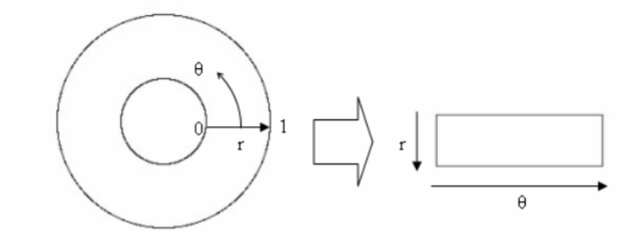
\includegraphics[width=0.90\textwidth]{img/daugman.png}
	\end{center}
	\legend{Fonte: \cite{masek2004}}
\end{figure}

O modelo resultante da aplicação do filtro de Daugman contem as informações da íris que serão utilizadas na identificação. A técnica utilizada no presente relatório utilizada a implementação proposta pro Libor Masek \cite{masek2004}, na qual o método de criação de \textit{template} da íris retorna, após a execução, um modelo no qual as técnicas de reconhecimento podem ser aplicadas. O chamado template biométrico codifica as características da imagem da íris. 
 
% ---
% ---------------------------------------------------------- % inclui o arquivo introducao.tex

% ----------------------------------------------------------


% ----------------------------------------------------------
% Fundamentação Teórica
% ----------------------------------------------------------

%\include{} % inclui o arquivo fundamentacao.tex

% ----------------------------------------------------------


% ----------------------------------------------------------
% Metodologia
% ----------------------------------------------------------

% ----------------------------------------------------------
% Metodologia
% ----------------------------------------------------------
\chapter{Experimentos}\label{cap:metodologia}
% ----------------------------------------------------------


% ----------------------------------------------------------
\section{Base de dados}\label{sec:bd}
% ----------------------------------------------------------

% ----------------------------------------------------------
\section{GLCM - \textit{Gray Level Co-ocurrence Matrix}}\label{sec:glcm}
% ----------------------------------------------------------

% ----------------------------------------------------------
\section{LBP - \textit{Local Binary Patterns}}\label{sec:lbp}
% ----------------------------------------------------------

% ----------------------------------------------------------
\section{Filtros de Gabor}\label{sec:gabor}
% ----------------------------------------------------------
 % inclui o arquivo metodologia.tex

% ----------------------------------------------------------


% ----------------------------------------------------------
% Desenvolvimento
% ----------------------------------------------------------
%% ----------------------------------------------------------
% Metodologia
% ----------------------------------------------------------
\chapter{Arquitetura do projeto}\label{cap:desenvolvimento}
% ----------------------------------------------------------
% ----------------------------------------------------------

A arquitetura implementada para o módulo de balanceamento segue a proposta apresentada na figura \ref{fig:arq}. O processo de desenvolvimento foi dividido em módulos: \textit{Load Balancer} (balanceador de carga), \textit{Neural Network} (Rede Neural), \textit{Request Server} (servidor de requisições) e \textit{Servers}, sendo os dois primeiros parte integrante do protótipo de balanceamento de carga e os dois últimos utilizados para teste do protótipo. 

O \textbf{módulo de \textit{servers}} é composto por dois servidores do tipo t2.micro, conforme descrito na tabela \ref{tab:servidores}, cada um deles configurado como um servidor que recebe requisições em uma porta especifica e retorna o conteúdo solicitado. O objetivo do módulo do balanceador de carga é distribuir a carga de requisições entre estes servidores. Para executar e configurar estes servidores, fez-se uso do Nodejs, com código semelhante ao apresentado na seção \ref{sec:node-js}, cujo acesso está ilustrado na figura \ref{fig:serv-req}. 
\begin{figure}[htb]
	\caption{\label{fig:serv-req}Conexão ao servidor de Requisições}
	\begin{center}
		\includegraphics[width=0.90\textwidth]{img/servidor.png}
	\end{center}
	\legend{Fonte: elaborada pela autora}
\end{figure}

O \textbf{módulo de servidor de requisições} simula um cliente. Seu algoritmo gera aleatoriamente uma quantidade de solicitações ao servidor de balanceamento e aguarda a resposta da requisição, gravando em um arquivo de \textit{log} se a solicitação foi atendida com sucesso. 

O último módulo é o protótipo de aplicação em si, composto por duas partes: a primeira, é responsável pelo algoritmo de distribuição das requisições e a segunda implementa a Rede Neural Artificial. 

O \textbf{módulo de balanceamento de carga} recebe todas as requisições geradas pelo módulo de requisições e distribui entre os servidores. Para efetuar esta distribuição, escolheu-se utilizar o conceito do algoritmo de Round Robin \cite{nginx-rr}, no qual as requisições são distribuídas entre os servidores seguindo a ideia de turnos, ou seja, em uma lista de servidores, o balanceador de carga direciona a requisição para o primeiro, a próxima para o segundo da lista e assim por diante, até atingir o último servidor da lista, reiniciando o \textit{loop}. A figura \ref{fig:round} ilustra essa distribuição. 
\begin{figure}[htb]
	\caption{\label{fig:round}Round Robin}
	\begin{center}
		\includegraphics[width=0.70\textwidth]{img/rrobin-01.png}
	\end{center}
	\legend{Fonte: elaborada pela autora}
\end{figure}

\textit{Round Robin} é um algoritmo que tem como principal vantagem a estabilidade e a simplicidade de implementação e execução. Porém, sua eficiência ou precisão não é tão grande quando comparada à abordagens mais complexas pois muitos balanceadores não consideram as diferenças entre os servidores que recebem as requisições \cite{nginx-rr}. Por esta razão, há variantes de implementações de \textit{Round Robin} que buscam minimizar esta desvantagem, dentre elas o \textit{Round Robin} com pesos e \textit{Round Robin} dinâmico. O primeiro, atribui pesos aos servidores associados na lista e a distribuição é feita com base nesse atributo. Servidores com maior peso recebem mais requisições. A segunda variante associa os pesos dinamicamente, de acordo com a carga atual e a ociosidade de cada servidor. 

O módulo de balanceamento de carga, então, utiliza o conceito de Round Robin com pesos, atribuindo pesos aos servidores do módulo de \textit{servers}. Os pesos são definidos com base no \textbf{módulo de Rede Neural}, descrito a seguir. Ainda em relação ao módulo de balanceamento, a implementação do protótipo incorpora os pesos atribuídos, ou  melhor, a classificação advinda da Rede Neural Artificial para executar o balanceamento. Este módulo também é responsável por atualizar as informações das características dos servidores, utilizadas posteriormente na Rede Neural. 

Por fim, o \textbf{Módulo de Rede Neural} implementa a rede responsável por atribuir os pesos aos servidores presentes na lista de servidores. As características consideradas no processamento dos pesos estão descritas na tabela \ref{tab:caracteristicas}. A saída deste módulo é ligada diretamente ao módulo de balanceamento, através de um vetor que indica quais servidores estão aptos a receber requisições. 

% ---
\section{Arquitetura da Rede Neural}\label{sec:ann}
% ---

A seção \ref{sec:rna} apresenta alguns modelos de arquiteturas que podem ser aplicadas para resolver problemas de classificação. Como discutido nesta mesma seção, a arquitetura do tipo de RNA ou abordagem utilizada para resolver um problema que envolva aprendizado está diretamente relacionada ao tipo de problema que se deseja resolver com determinada técnica. Este trabalho tem definido em seus objetivos aplicar uma Rede Neural Artificial para aprender se os servidores gerenciados pelo \textbf{módulo de balanceamento} estão aptos a realizar uma requisição. 

Como discutido na seção \ref{sec:balanceamento-carga}, este tipo de aplicação deve considerar elementos como distribuição esparsa da arquitetura em núvem, capacidade de armazenamento, complexidade do algoritmo e pontos de falhas, tempo de resposta, utilização de recursos, dentre outros critérios que determinam a eficiência de uma aplicação de balanceamento. 

Diante do problema, este trabalho considerou que, ao incorporar ao algoritmo de balanceamento uma RNA, um critério crucial para a escolha de sua arquitetura está diretamente ligada às características citadas anteriormente. Portanto, elementos como tempo de resposta e complexidade do algoritmo receberam certa prioridade em relação ao desempenho da rede na classificação em si. Como discutido na seção \ref{sec:rna}, a escolha da arquitetura, suas funções de ativação, tipo de aprendizado, e, principalmente, número de camadas e neurônios, são características que impactam diretamente no tempo de processamento. Redes com muitas camadas, como as CNNs, por exemplo, levam um tempo consideravelmente alto no aprendizado e possuem uma arquitetura sofisticada. 

Considerando que a RNA escolhida seria incorporada ao \textbf{módulo de balanceamento} e que, por ser uma aplicação de balanceamento de carga de requisições - onde o tempo de resposta é importantíssimo - o modelo escolhido foi o Perceptron, por ser de simples implementação. Além disso, a definição das características também permitiu que este modelo se apresentasse como uma boa escolha, visto que o número de características é pequeno e o problema de classificação, neste caso, não exige uma função tão complexa de separação dos dados no espaço de características. 

Portanto, este trabalho considerou como critério de escolha da rede a simplicidade da implementação da RNA para diminuir a complexidade do \textbf{módulo de balanceamento}, dimensão do problema (em relação às suas características) e tempo de resposta. Tendo isto em vista, o modelo escolhido foi o Perceptron e a arquitetura da rede está descrita a seguir. 

% ---
\textbf{Definição de características}

A tabela \ref{tab:caracteristicas} descreve as características que a RNA recebe como \textit{input}. Cada uma delas impacta diretamente no desempenho da distribuição das requisições. O tipo de servidor, apesar de ser um parâmetro estático (ou seja, não muda ao longo da execução), quando colocado em conjunto com as demais características, torna-se importante. Por exemplo, um servidor que possui maior capacidade de processamento e está à uma distância maior do que um servidor com menor capacidade e mais próximo pode ter um tempo de resposta semelhante, equilibrando o peso do servidor em relação aos demais. 

\begin{table}[h]
	\caption{Características}
	\centering
	\small
	\renewcommand{\arraystretch}{1.2} % Aumenta espaçamento vertical
	\begin{tabular}{>{\centering\arraybackslash}m{3.5cm} m{11.5cm}}
		\hline 
		\textbf{Característica} & \textbf{Descrição}  \\ 
		\hline 
		\textbf{Tipo de servidor}& t2.micro ou t2.medium - servidores com maior poder de processamento podem receber um número maior de requisições \\ 
		\hline 
		\textbf{Tempo de resposta } & Tempo para receber e responder à requisição\\ 
		\hline 
		\textbf{Estado} & Indica se o servidor está apto à receber requisições\\ 
		\hline 
		\textbf{Distâcia} & Atribui um valor de distância (física) para o servidor - Neste caso, servidores mais distantes demoram mais para responder\\ 
		\hline 
	\end{tabular}\\
	\vspace{3mm}
	\legend{Elaborado pela autora.}
	\label{tab:caracteristicas}
\end{table}

Características como tempo de resposta e estado são dinâmicas, ou seja, mudam ao longo da execução do algoritmo. Essas características impactam diretamente na decisão, visto que, um servidor que recebe muitas requisições (ou seja, está sobrecarregado) em uma iteração pode, na seguinte, estar livre, caso consiga responder à todas as requisições em sua fila. 
A discussão acerca da escolha destas características e sua efetividade é apresentada no capítulo de \ref{cap:resultados}.

% ---
\textbf{Implementação da Rede Neural com Perceptron}


A Rede Neural escolhida segue a ideia de Perceptron apresentada na seção \ref{sec:rna}. A rede contem três camadas: uma de entrada, uma escondida e uma camada de saída. Por se tratar de uma rede neural aplicada à balanceamento de carga, alguns conceitos foram levados em conta ao estabelecer a forma de aprendizado dinâmico.Pelas razões elencadas no início desta seção, a rede neural escolhida possui poucas camadas, como ilustrado pela figura \ref{fig:rede}, com o objetivo de aumentar a velocidade de processamento e garantir que o tempo de resposta do balanceador não seja tão afetado pelo tempo de processamento da RNA. Além disto, a quantidade de características e o tipo de saída esperada na arquitetura proposta por este projeto permitem uma implementação de uma rede deste tipo. 

\begin{figure}[htb]
	\caption{\label{fig:rede} Camadas implementadas na rede neural}
	\begin{center}
		\includegraphics[width=0.60\textwidth]{img/redeusada.png}
	\end{center}
	\legend{Fonte: elaborada pela autora}
\end{figure}

A primeira camada presente na arquitetura da rede neural é a camada de entrada. É composta por um vetor $x$ de tamanho $n$, sendo $n$ igual ao número de características (apresentadas na tabela \ref{tab:caracteristicas}) do servidor. Os pesos que essas características tem na classificação são armazenados em $w$. Em teoria, $w$ consiste em uma matriz que possui $n$ linhas (quantidade de \textit{inputs}) e $m$ colunas (quantidade de \textit{outputs}). Como a saída é a classificação se o servidor está apto à receber a requisição, ou seja, o \textit{output} da rede é a classificação como "apto" ou "não apto", um único neurônio nesta camada é suficiente, logo, neste caso, $w$ passa a ser um vetor de pesos. 

As sinapses ou propagação de sinal da primeira camada para a segunda é feita seguindo o cálculo na equação \ref{eq:pesos}. 
\begin{equation}
x_i = x_i \times w_i
\label{eq:pesos}
\end{equation}

A segunda camada realiza um somatório das características (\ref{eq:sum}) e aplica a função sigmoide da equação \ref{eq:sigmoide} ao resultado. $y_j$ é a variável que guarda o valor do somatório da iteração $j$. Antes de aplicar a sigmoide, os valores são multiplicados por 0.02 para diminuir a faixa de valores na saída. 

\begin{equation}
y_j = \sum_{i=1}^{n} {x_i}
\label{eq:sum}
\end{equation}


\begin{equation}
S(y_j) =  \frac{1}{(1 + e ^ {y_j} )} 
\label{eq:sigmoide}
\end{equation}

A última camada utiliza o \textit{output} para ajustar os pesos em $w$. Esta é a fase de treinamento da rede, que ocorre de maneira dinâmica. Ao fim da classificação, o \textit{output} identifica o servidor como "apto" ou "não apto" a receber requisições. Se for classificado como "apto", e a requisição for direcionada para ele então a classificação foi correta o algoritmo ajusta o peso que mais influenciou a decisão, seguindo a equação \ref{eq:weight}. Caso a classificação seja incorreta, e a requisição retornou uma falha ou o servidor não conseguiu atender a requisição, o ajuste de peso diminui o peso da característica que mais influenciou a decisão, seguindo a equação \ref{eq:weight2}

\begin{equation}
w_i = w_i + 0.5
\label{eq:weight}
\end{equation}

\begin{equation}
w_i = w_i - 0.5
\label{eq:weight2}
\end{equation}

Ao fim do processamento, os valores de $w$ são salvos para uso posterior. A ideia de manter o treinamento constante da rede advém de sua implementação mais simples, que permite velocidade no processamento e atribuição dos valores de pesos utilizados pelo balanceador de cargas, visto que os as entradas mudam de maneira rápida e o treinamento depende dos resultados anteriores. 

% ---
\section{Implementação e Testes}\label{sec:testes}
% ---

Por se tratar de uma aplicação de \textit{backend} implementada em Nodejs, o protótipo não possui interface gráfica, de modo que sua interface de comandos é feita pelo terminal, como pode ser observado na Figura \ref{fig:consoleann}. Ao iniciar o acesso, o balanceador verifica quais servidores estão ativos e os coloca em uma lista, como apresentado na Figura \ref{fig:areas}. Então, a aplicação verifica a conexão com cada um dos servidores na lista, para garantir que o mesmo possui o estado saudável. 

Em seguida, são atribuídas os valores das características para cada servidor na lista, seguindo a definição apresentada na tabela \ref{tab:caracteristicas}. Caso seja a primeira vez que a aplicação de balanceamento é executada, $w$ é preenchido com valores padrões. Caso contrário, dados salvos em um arquivo que guarda as informações de peso do processamento anterior são carregados. 


A implementação foi feita em Nodejs e o código está disponível no Github\footnote{\url{https://github.com/ksetoue}} da autora. O algoritmo implementado para balanceamento de cargas com a rede neural segue os seguintes passos: 
\begin{enumerate}
	\item \textit{inicialização de paramêtros}: inicialização do vetor de pesos, objeto que armazena dados dos servidores;
	\item \textit{se nova requisição recebida}: 
	\begin{enumerate}
		\item classificar cada servidor (chamar a RNA)
		\item escolher a melhor opção para direcionar a requisição 
		\item verifica se a requisição foi atendida 
		\item manda o resultado para o cliente 			
	\end{enumerate}
	\item \textit{Ajustar os pesos}: conforme descrito em \ref{sec:ann};
	\item \textit{Caso desativado}: salvar paramêtros de peso; 
	\item \textit{Senão}: voltar ao primeiro item; 
\end{enumerate}

As figuras \ref{fig:consoleann}, \ref{fig:areas} e \ref{fig:weights} apresentam a interface no console da aplicação de balanceamento em execução. As informações apresentadas são a lista de servidores ativos e os pesos mais recentes. 

\begin{figure}[htb]
	\caption{\label{fig:consoleann} \textit{Screenshot} de teste realizado com a Rede Neural}
	\begin{center}
		\includegraphics[width=0.70\textwidth]{img/load-bal-app.png}
	\end{center}
	\legend{Fonte: elaborada pela autora}
\end{figure}

Esta parte da aplicação corresponde ao \textbf{módulo de balanceamento}, executado no servidor t2.medium. 

\begin{figure}[htb]
	\caption{\label{fig:areas} \textit{Screenshot} Dados do Balanceador - Servidores Ativos}
	\begin{center}
		\includegraphics[width=0.80\textwidth]{img/activeservers.png}
	\end{center}
	\legend{Fonte: elaborada pela autora}
\end{figure}

\begin{figure}[htb]
	\caption{\label{fig:weights} \textit{Screenshot} Dados do Balanceador - Pesos mais recentes (RNA)}
	\begin{center}
		\includegraphics[width=0.50\textwidth]{img/weights.png}
	\end{center}
	\legend{Fonte: elaborada pela autora}
\end{figure}





 % inclui o arquivo desenvolvimento.tex

% ----------------------------------------------------------
% Resultados
% ----------------------------------------------------------
% ----------------------------------------------------------
% Desenvolvimento
% ----------------------------------------------------------
\chapter{Resultados}\label{cap:resultados}
% ----------------------------------------------------------

 % inclui o arquivo resultados.tex

% ----------------------------------------------------------


% ----------------------------------------------------------
% Conclusão
% ----------------------------------------------------------
\chapter{Conclusão}
% ---------------------------------------------------------- 

As implementações podem ser encontradas em https://github.com/ksetoue/iris

% ----------------------------------------------------------

% ----------------------------------------------------------------------------------------------------------------------------------



% ----------------------------------------------------------
% ELEMENTOS PÓS-TEXTUAIS
% ----------------------------------------------------------

% ----------------------------------------------------------
% Referências bibliográficas
% ----------------------------------------------------------
\bibliography{referencias}
% ----------------------------------------------------------


\end{document}
